\section{Movimiento Rectilíneo Uniforme (MRU)}
El Movimiento Rectilíneo Uniforme (MRU) es aquel en el que un objeto se desplaza en línea recta con velocidad constante, es decir, con aceleración igual a cero.

\begin{figure}[htbp]
    \centering
    \adjustbox{margin={0pt 10pt 0pt 0pt}}{
        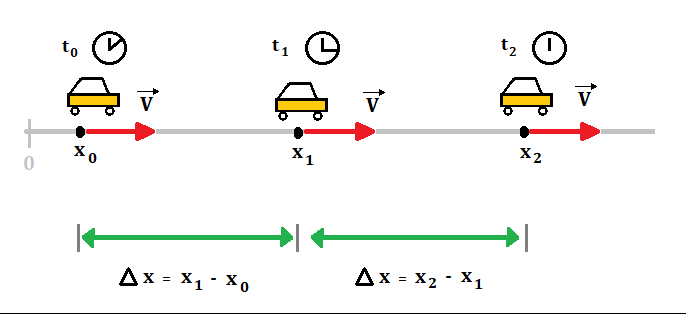
\includegraphics[width=0.8\textwidth, trim=0 5 0 0, clip]{images/cinematicImages/uniformRectilinearMotion.png}
    }
    \caption{Representación gráfica del movimiento rectilíneo uniforme}
\end{figure}

\vspace{-40pt}

\[
a = 0 \qquad v = \text{constante}
\]

\subsection{Ecuación de posición}

{v} = \text{ctte} \quad \text{la velocidad no es función del tiempo}
\begin{align*}
\text{* la ecuación integral}\\
\int_{x_0}^{x} dx &= \int_{t_0}^{t} v(t)\, dt\\
\text{* si } v(t)=\text{ctte}=v\\
\int_{x_0}^{{x^0}} {x^0} dx &= v \int_{t_0}^{t} {t^0} dt\\
\left[\frac{1}{0+1}x^{0+1} \right]_{x_0}^{x} &= v\left[\frac{1}{0+1}t^{0+1}\right]_{t_0}^{t}\\
[x]_{x_0}^{x} &= v[t]_{t_0}^{t}\\
x - x_0 &= v(t - \cancel{t_0})\\
\end{align*}

\vspace{-60pt}

\begin{align*}
    \hspace{1.8cm} \Aboxed{x &= x_0 + vt}
\end{align*}

Donde:
\begin{itemize}
    \setlength{\itemsep}{0pt}
    \item $x$: posición final
    \item $x_0$: posición inicial
    \item $v$: velocidad constante
    \item $t$: tiempo transcurrido
\end{itemize}

\subsection{Características del MRU}

\begin{itemize}
    \setlength{\itemsep}{0pt}
    \item La trayectoria es una línea recta.
    \item La velocidad se mantiene constante en módulo, dirección y sentido.
    \item La aceleración es cero.
    \item El desplazamiento es proporcional al tiempo.
\end{itemize}
